\chapter{$K^0$ 2-step and Direct-$\Lambda(1520)$ production}
\section{Template fitting}
\begin{figure}[htbp]
  \centering
  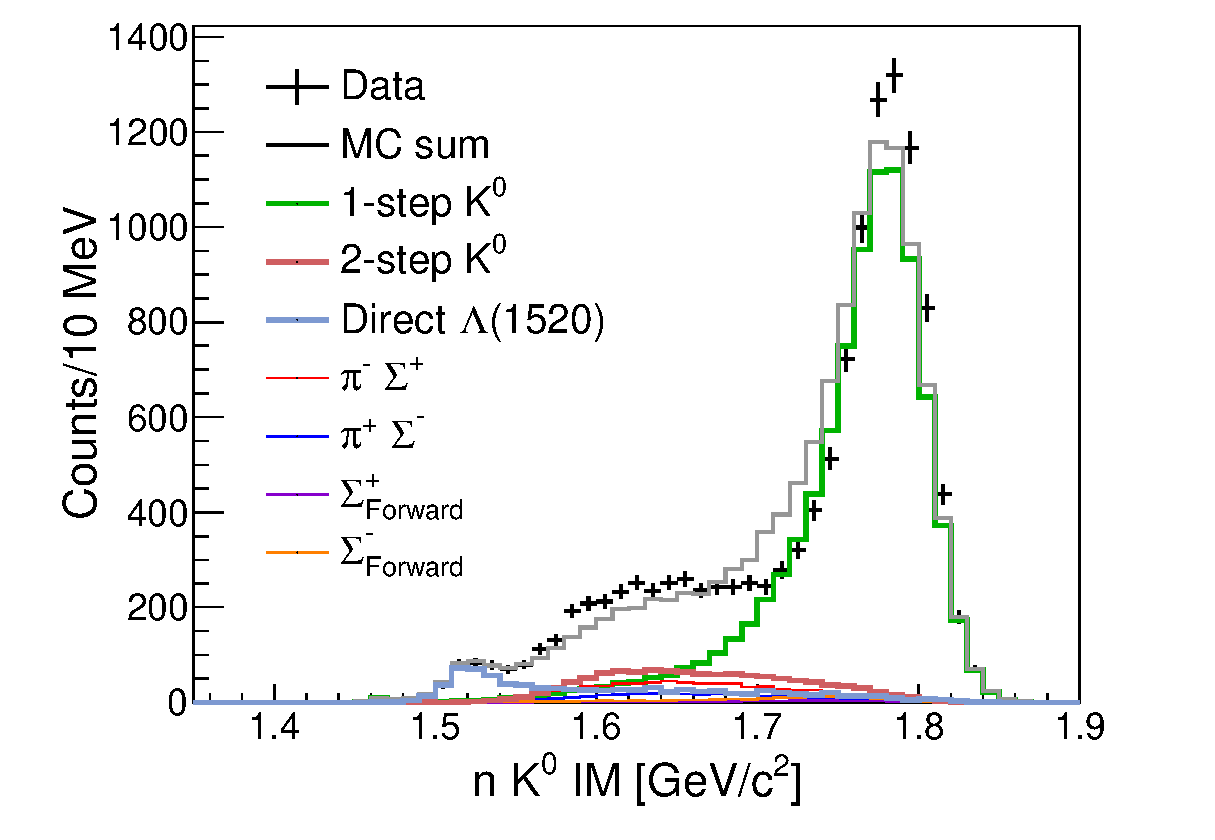
\includegraphics[width=8cm]{../pic/Dron/K0_ana/npipi_IM_K0.eps}
  \caption{
    The figure shows $n K^0$ invariant masses and template fitting for the reaction decomposition of $K^0$ production events.
    Error bars indicate data.
    Bold lines indicate MC sim for 1-step $K^0$, 2-step $K^0$, and direct $n\Lambda(1520)$ production reactions in green, dark red, and dark blue, respectively.
    Thin lines indicate background events in $K^0$ production reactions, backward $\pi^- \Sigma^+$, backward $\pi^+ \Sigma^-$, $\Sigma^+_{forward}$, and $\Sigma^-$ in red, blue, purple, and orange.
  }
  \label{fig:fit_nK0_IM}
\end{figure}

In quasi-elastic scattering, the momentum of the spectator is small due to the Fermi motion of the spectator.
Therefore, the scattered $K^0 n$ has almost all the energy, so the invariant mass is distributed around the kinematic threshold.

However, our experimental data, represented by the error bars in Fig.\ref{fig:fit_nK0_IM}, have widely distributed components.
The spectra reproduced in the MC simulations are also plotted as coloured lines in the same figure.
The bold line shows the actual K0-produced signal, while the green line indicates 1-step quasi-elastic scattering.
The two other dark red and dark blue lines indicate 2-step and direct $\Lambda(1520)$ production, which will be discussed in more detail below.
The thin coloured lines represent the background,
with red, blue, purple and orange indicating backward $\pi^- \Sigma^+$, backward $\pi^+ \Sigma^-$, $\Sigma^-_{forward}$ and $\Sigma^+_{forward}$, respectively.

In the 2-step $K^0$ reaction, the recoiled $K^0$ scatters with residual nucleons and shares its energy with them.
Therefore, the invariant mass of n K0 is widely distributed in the allowed kinematic region.
A bump structure is observed near $\Lambda(1520)$, indicating that $K^- d \rightarrow n \Lambda(1520)$ reaction and $\Lambda(1520)\rightarrow n K^0 $decay are taking place.
As a result of this template fit, the $-2\log \Lambda$ is estimates as $\KzeroFitChi$ and $NDF$ is $\KzeroFitNDF$, so $-2\log \Lambda/NDF \sim \KzeroFitChiNDF$.
The, the ratio of 1-step to true $K^0$ production excluding background is estimated to $\KzeroOneStepRatio$, 2-step $\KzeroTwoStepRatio$ and direct-$\Lambda(1520)$ $\KzeroLsRatio$.

\section{Affect to the $d(K^-, n)$ Spectra}
\begin{frame}{$d(K^-, n)"n K^0"$運動量カット}

\end{frame}

We explain effect of these reactions contaminating into the main signal, $d(K^-, n)"\pi^{\mp}\Sigma^{\pm}"$, as background.
Fig.\ref{fig:KN_MM_K0} shows the $d(K^-, n)$ missing mass with $K^0$ identified.
The data is represented by error bars with the MC where the K0 was actually created by a bold line and the background by a thin line.
Since the spectral shape of $d(K^-,n)$ is determined by the initial $\bar{K}N$ scattering, the 2-step reaction is almost identical to the 1-step reaction.
On the other hand, the direct $\Lambda(1520)$ production makes a bump structure on $d(K^-, n)$ too.
Since the contribution of this reaction is so small, this background effect is almost no change.

\section{Conversion to the Cross Section}
\begin{frame}{$K^0 cos\theta$ vs mom  {\bf Data}}
  \begin{tabular}{cc}
    \begin{minipage}{0.5\hsize}
      \begin{figure}
        Raw\\
        \includegraphics[width=6cm]{../pic/Run78/QE/K0_cos_mom_data.eps}
      \end{figure}
    \end{minipage}

    \begin{minipage}{0.5\hsize}
      \begin{figure}
        $Data(\cos_{K^0}, p_{K^0}))/A(\cos\theta_{K^0}, p_{K^0})$\\
%%        Accpectance corrected\\
        \includegraphics[width=6cm]{../pic/Run78/QE/K0_cos_mom_data_corr.eps}
      \end{figure}
    \end{minipage}
  \end{tabular}
  
  \centering

  Acceptance was presented at page.4
  
\end{frame}

\subsection{The spectrum of the $d(K^-, n)"n K^0"$}

\begin{figure}
  \centering
  \begin{tabular}{cc}
    \begin{minipage}{0.6\hsize}
      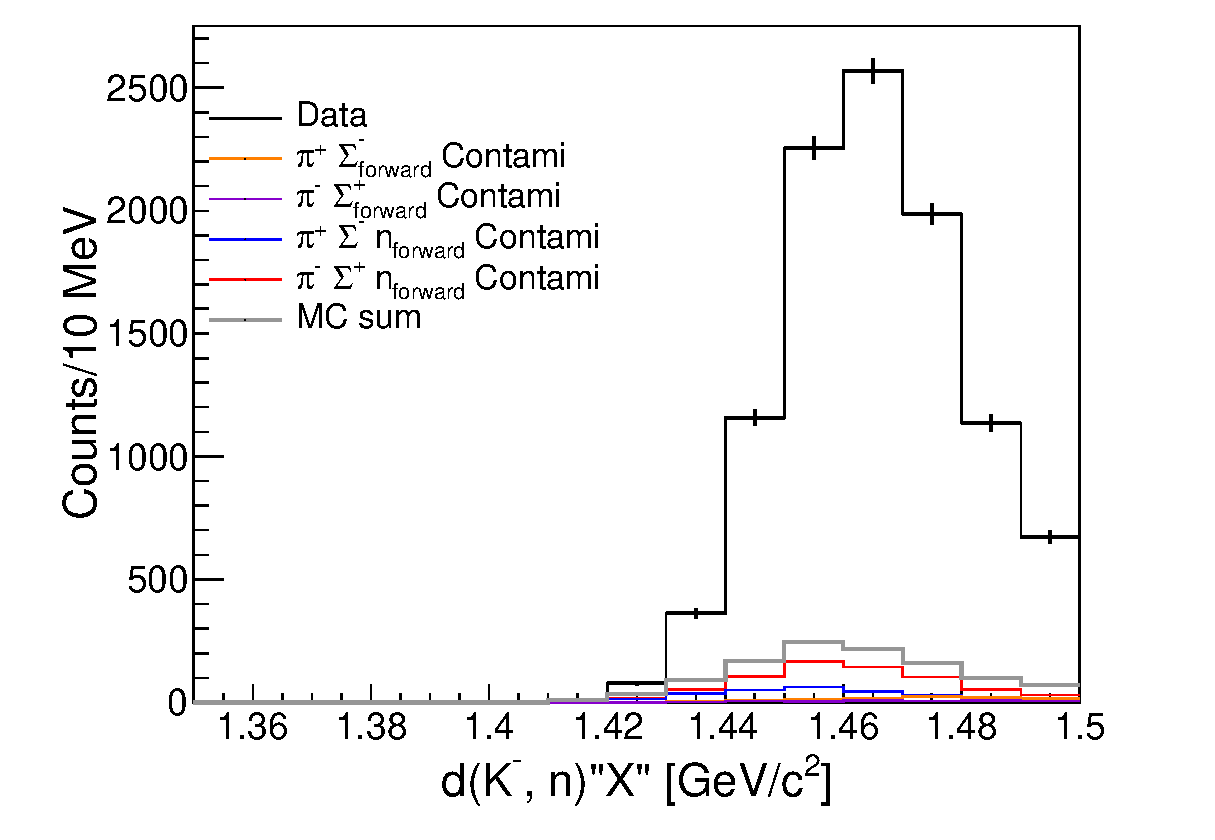
\includegraphics[width=7cm]{../pic/Run78/QE/KN_MM_wK0_tag.eps}
    \end{minipage}
    \begin{minipage}{0.4\hsize}
      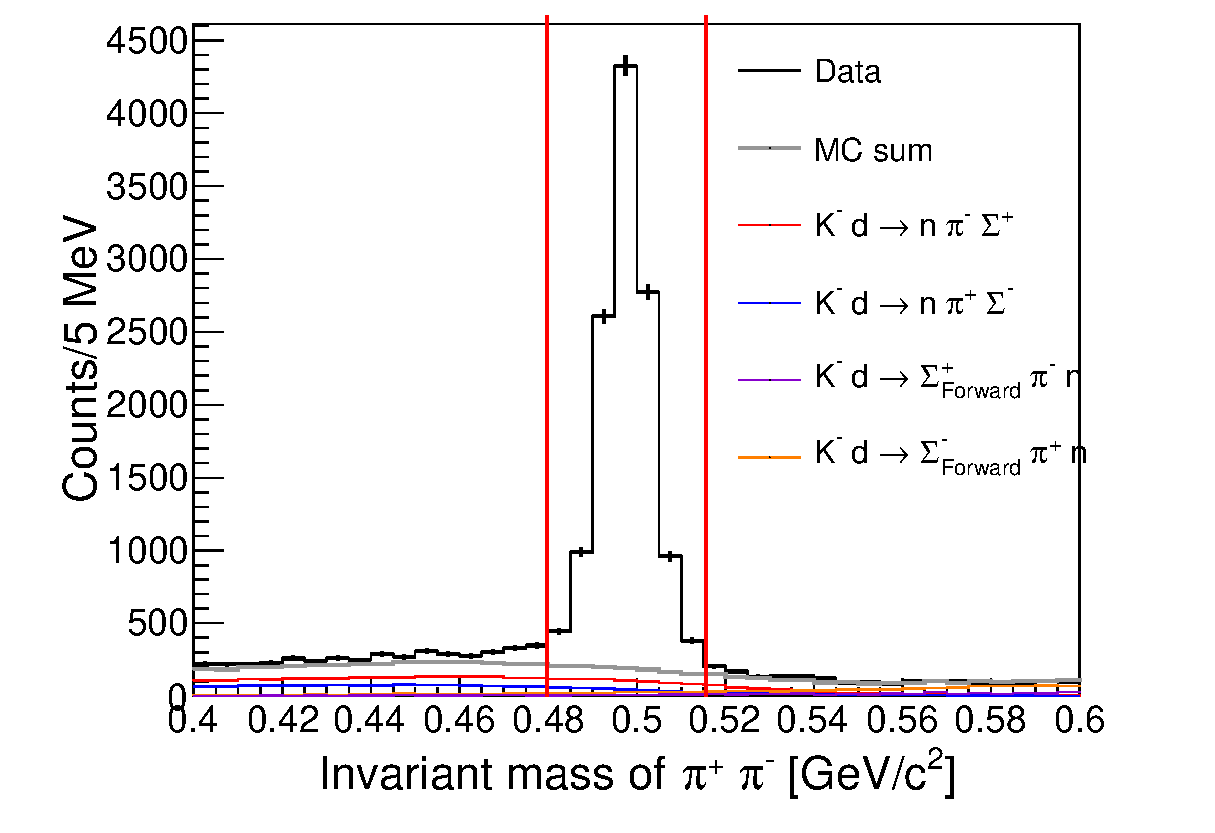
\includegraphics[width=4cm]{../pic/Run78/QE/IM_pipi.eps}
    \end{minipage}
  \end{tabular}
  \caption{
    Right figure shows $K^0$ selection region and estimated background events which is zoom up of left figure of Fig\ref{fig:IM_fit}.
    Red lines indicate selection region.
    left figure shows $d(K^-, n)"n K^0"$ spectra with esmated backgrounds by MC template.
  }
  \label{fig:KN_MM_K0}
\end{figure}

Although the reaction can not measured below the $\bar{K}N$ threshold, 
in the $K^0$ take the strangeness, 
so these events are one of the strongest candidate of the prove for 1-step reaction strength of the $K^-N\rightarrow \bar{K}n$ reaction.\\
The backgrounds were estimated using the template fitting result which was shown in the right figure of Fit\ref{fig:KN_MM_K0}.
The background spectra shape of the $d(K^-, n)"n K^0"$ was indicated in the left figure of the same figure.
These spectra will be collected by the acceptance of the CDS using	the $K^0$ kinematics because detected particles by the CDS came from the $K^0$ decay.
The $K^0$ kinematics was represented as 2 variables function about the $\cos\theta$ and the absolute momentum value and
the acceptance of the CDS was collected event-by-event using the acceptance as weight function as the following equation.

\begin{equation}
  N_{corr}(m_{n K^0}) = \sum N(m_{n K^0}, \cos\theta_{K^0}, p_{K^0}) \cdot \frac{1}{A(\cos\theta_{K^0}, p_{K^0})} \label{eq:corr_K0} 
\end{equation}

\begin{figure}[htbp]
  \centering
  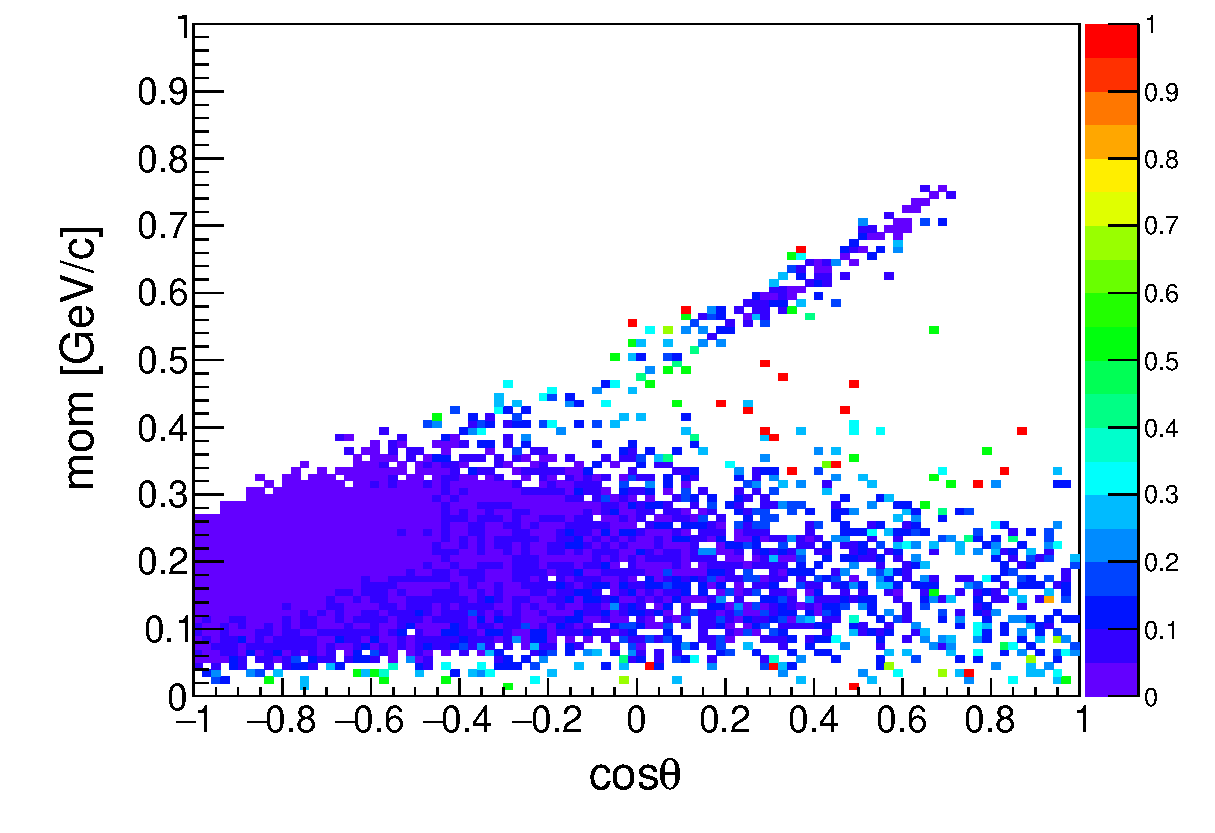
\includegraphics[width=7cm]{../pic/Run78/QE/K0_cos_mom_acc.eps}
  \caption{
    This figure shows the acceptance of the $K^-d\rightarrow K^0 n n$ reaction which was estimated by the Monte Calro simulation.
  }
  \label{fig:K0_acc}
\end{figure}

\begin{figure}[htbp]
  \centering
  \begin{tabular}{cc}
    \begin{minipage}{0.5\hsize}
      \includegraphics[width=7cm]{../pic/Run78/QE/K0_cos_mom_data.eps}
    \end{minipage}

    \begin{minipage}{0.5\hsize}
      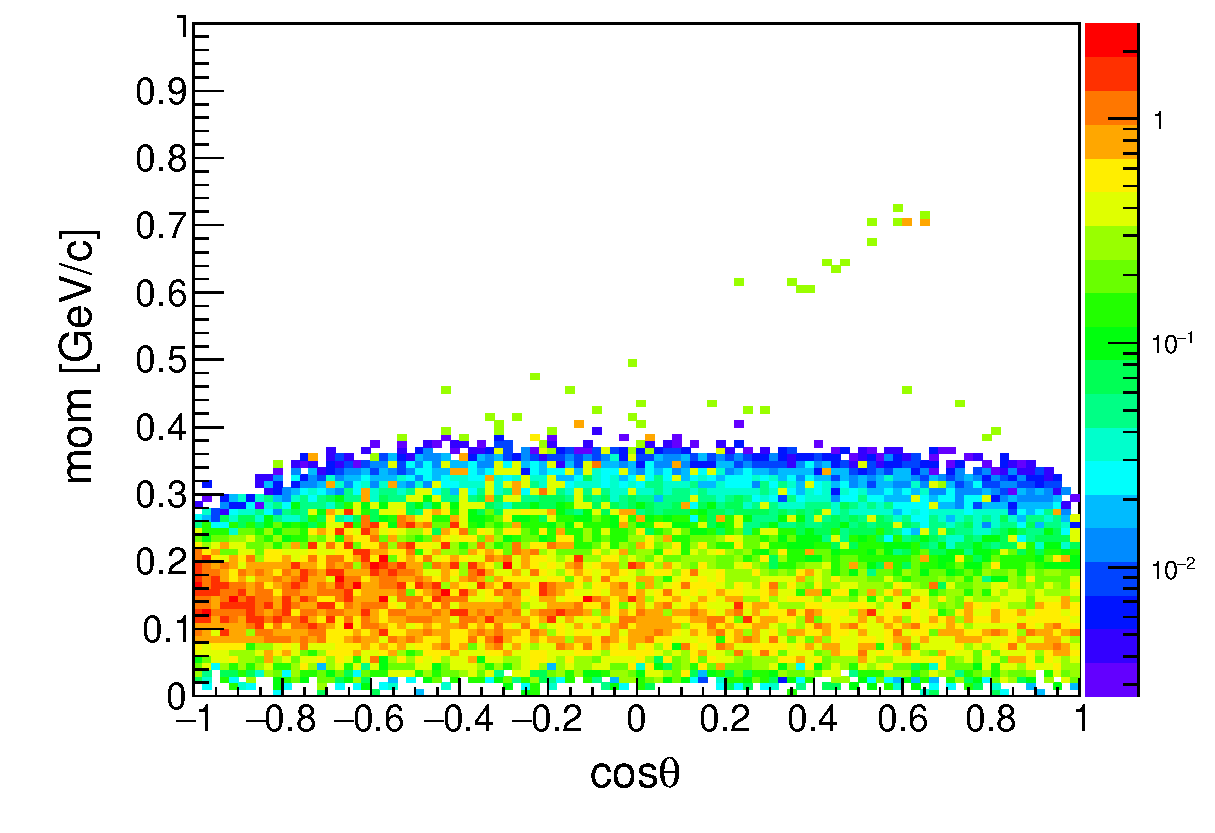
\includegraphics[width=7cm]{../pic/Run78/QE/K0_cos_mom_BG.eps}
    \end{minipage}
  \end{tabular}
  \caption{
    These figure shows about $K^0$ emit angle and momentum in the experimental frame.
    Left figure shows about data and right figure shows background estimated by the Monte Calro.
  }
  \label{fig:K0_cos_mom}
\end{figure}

For this collection, the acceptance was estimated using the $K^- d \rightarrow n_{forwad} (K^0 n)$ reaction.
The mass of the $n K^0$ was generated flat distribution from the $K^0 n$ mass threshold to the kinematical threshold
to accumulate widely and isotropically acceptance which was shown in Fig\ref{fig:K0_acc}
This acceptance collection was adopted to the signal and the backgrounds.
Fig\ref{fig:K0_cos_mom} shows the $K^0$ kinmatics distribution about the data and the backgrounds estimated by the MC sim.
By this operation, we obtained the acceptance collected spectra as shown in Fig\ref{fig:KN_MM_K0_corr}.
Because the data distribution located at the edge of the acceptance and the backgrounds widely distributed, in the acceptance corrected spectra, the signal was enhanced.

\begin{figure}[htbp]
  \centering
  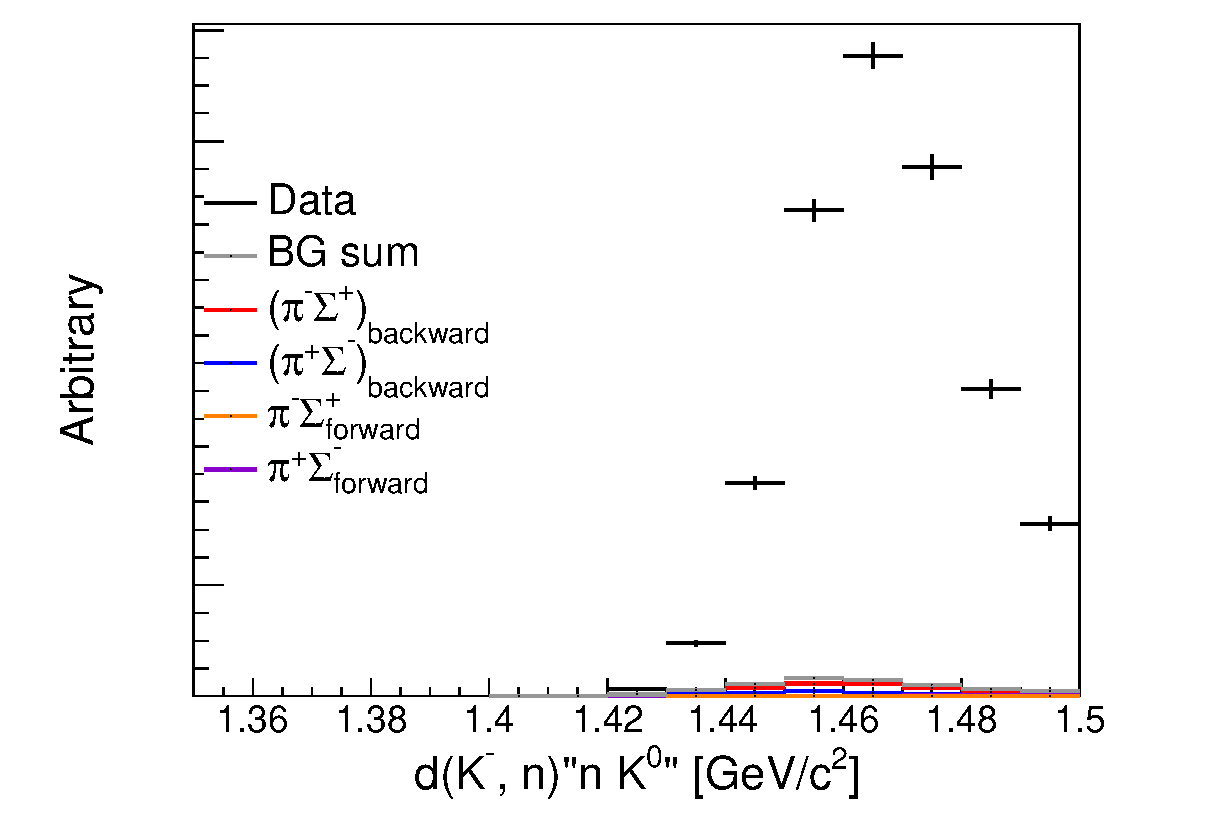
\includegraphics[width=8cm]{../pic/Run78/QE/K0_spec_wBG.eps}
  \caption{
    This figure shows acceptance corrected spectrum of the $d(K^-, n)"n K^0"$.
    Black line indicates data and color plots indicate the background reproduced by the Monte Calro simulation.
  }
  \label{fig:KN_MM_K0_corr}
\end{figure}


For $K^0$ production events, we use acceptance for $K^0$ kinematics because all detected particles are of $K^0$ origin.
We estimate the two-dimensional acceptances for $K^0$ momentum and $K^0$ scattering angles as shown in Fig\ref{fig.K0_cos_mom_acc}, and weight each event to correct for acceptances.
Fig.\ref{fig:K0_spec} shows acceptance corrected spectra of $K^0$ production with reproduced BG by MC simulations.
It can be seen that the data are concentrated in the backward and high momentum regions where the acceptances are small,
while the MC is distributed over the whole region as shown in Fig.\ref{fig:K0_cos_mom}.
In other words, the acceptance correction suppresses BG and emphasizes true $K^0$ production.

Multiplying the obtained spectra by the conversion factor discribed in Sectrion.\ref{sec:conversion_factor} yields the cross sections shown in Fig.\ref{fig:nK0_CS}.
The $d(K^-,n)"nK^0"$ spectra do not contain information below the $\bar{K}N$ threshold but are suitable for studying the $d(K^-, n)$ reaction.
This spectrum is similar to the bump structure of the so-called quasi-elastic scattering.
This spectrum contains about 12\% of the 2-step reaction described in the previous section.
Since the missing mass of $d(K^-,n)$ is determined by the $K^- N \rightarrow \bar{K}N$ scattering of the first reaction, this spectrum has almost the same shape as quasi-elastic scattering.
The strength of the 2-step at the quasi-elastic scattering bump is $35 mb/\Omega \cdot \mbox{MeV}$, which is consistent with $d(K^-, N)"\pi \Sigma"$ in order.

\begin{frame}{Cross Section of $d(K^-, n)"n K^0"$}
  \begin{figure}
    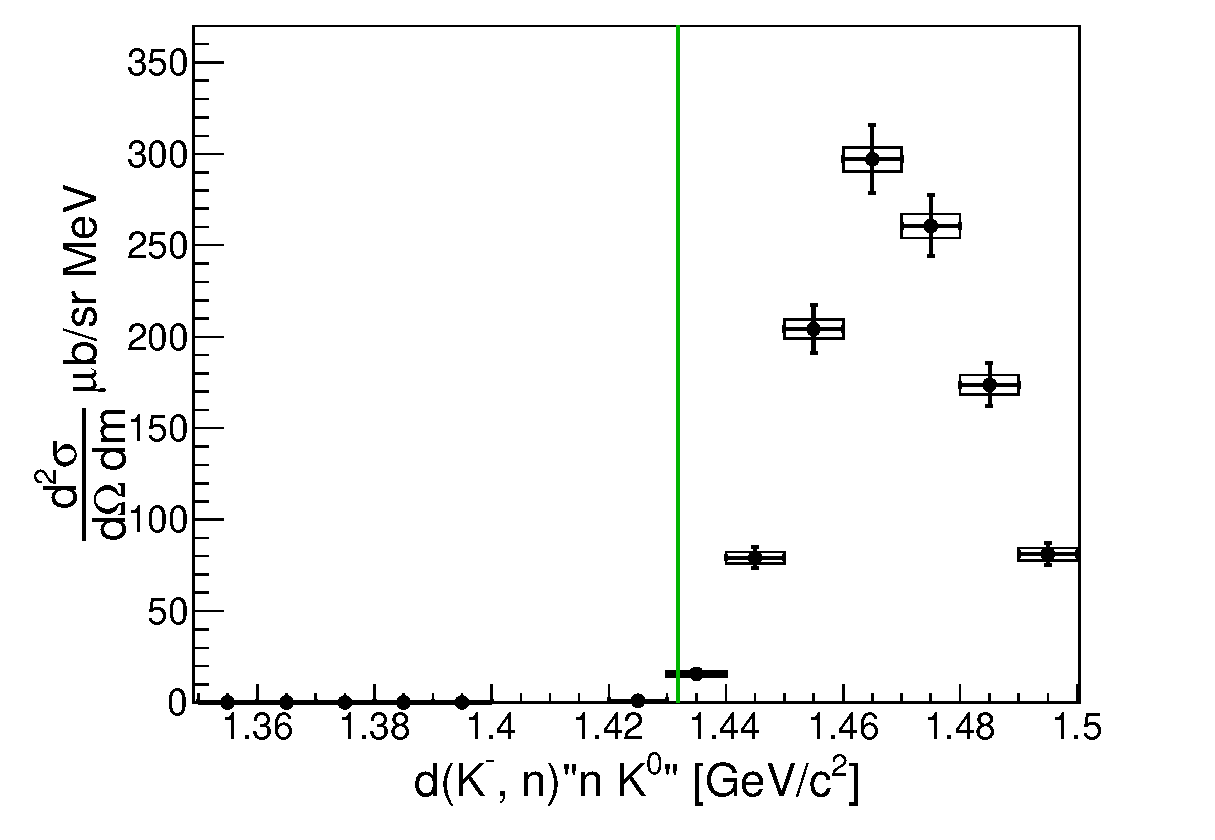
\includegraphics[width=8cm]{../pic/Run78/QE/K0_CS.eps}
  \end{figure}
  \centering
  Box indicates staticial errors.
%%  BG was subtracted.
\end{frame}

